\chapter{Applications of Word-Level Abstraction of Galois Field 
Circuits}
\label{ch:prop}

In this chapter, we propose two additional applications of word-level 
abstractions
of Galois field circuits. First, we propose an approach to partition
any Galois field arithmetic circuit over $\Fkk$ into sub-circuit  
blocks, each of which can then be analyzed over the same field $\Fkk$.
As each block is a smaller partition of the overall circuit, the 
abstraction complexity of each partition is smaller. Thus, 
word-level abstraction
of the sub-circuits is faster than abstraction of the original circuit.
Abstraction of each sub-circuit can be performed independent of each other,
after which the word-level representations can be combined to find the 
overall function of the entire circuit.
Second, we propose a method for applying our abstraction approach to 
combinational circuits whose function maps one Galois field to 
a different one,
i.e. $f:F_{2^k} \rightarrow F_{2^j}$ where $k \neq j$.

\section{Partitioning Algorithm}
Galois field arithmetic circuits of practical sizes are very large.
As the size of these circuits increase, the computational complexity of a
word-level abstraction increases exponentially.

However, if a large circuit is partitioned, that is 
seperated into smaller seperate pieces, the complexity of each partition is 
smaller and and thus each partition is more manageable.
For word-level abstraction of a circuit, an abstraction of each partition
could be performed and then the word-level representations could be combined
to find the overall word-level representation on the entire circuit.
In addition, each piece
could be abstracted in parallel, thus decreasing the time to
find the overall abstraction.
Recall our abstractions results of the Montgomery multiplier circuits, shown
in Table \ref{tab:absmontflatresults} for a 'flat' abstraction
and Table \ref{tab:absmontresults} for block abstractions. The Montgomery
circuit structure is shown in Figure \ref{fig:montmont}.

\begin{figure}[H]
	\begin{center}
	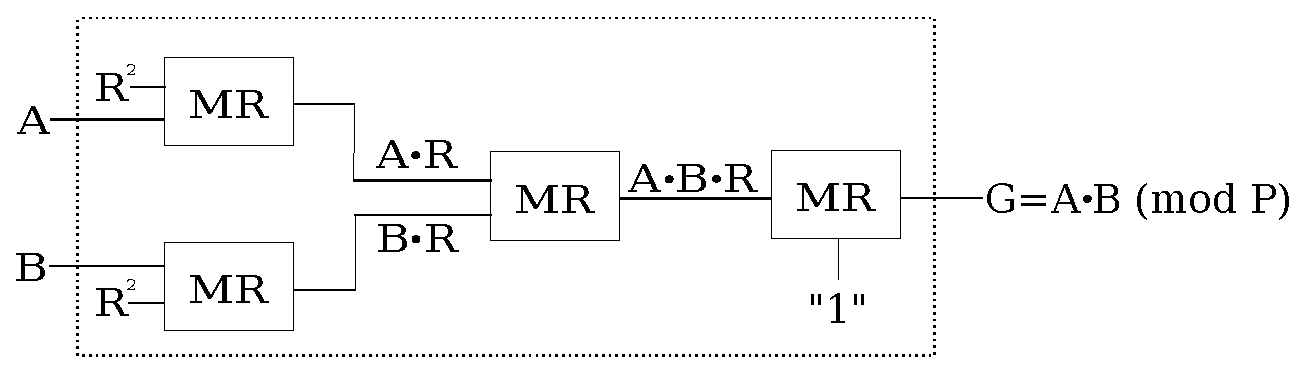
\includegraphics[scale=0.50]{figures/mmcircuit}
	\end{center}
	\caption{Montgomery multiplier over $\mathbb{F}_{2^k}$}
	\label{fig:montblock}
\end{figure}

Each block of the multiplier could be considered a partition. By 
comparing our results for the flat multiplier to the results of each 
block, the power of partitioning becomes apparent. Since the block 
abstractions can be performed in parallel, the time for an 
overall word-level abstraction is based on the time of the slowest block
abstraction.

\subsection{Partition Problem Statement}

The goal of our proposed partitioning algorithm 
is to quickly find partitions for any circuit. 
Given a circuit over $\Fkk$, each partition must have $k$-bit inputs and 
one $k$-bit output for simplicity in calculation.
These restrictions allow us to calculate the polynomial representation of 
each partition over the same field $\Fkk$. Thus, our problem statement is
as follows:

\begin{itemize}
\item Given a Galois field $\Fkk$, i.e. given the corresponding
irreducible polynomial $P(x)$ in $\F[x]$ of degree $k$,
let $P(\alpha) = 0$ where $\alpha \in \Fkk$ is the root of the irreducible
polynomial $P$.
\item  Given a gate-level combinational circuit $C$ with $n$ word-level
$k-bit$ inputs,
$A_1,\dots, A_n \in \Fkk$
and one $k-bit$ output $Z \in \Fkk$.
\item The bit-level primary inputs of the circuit are denoted
$\{a_{0}^{i},a_{1}^{i},\dots,a_{k-1}^{i}\}$, for $i=1,\dots, n$;
the primary bit-level outputs are $\{z_0, \dots, z_{k-1}\} = Z$. 
Note that all $a_{i}^{j}, z_i \in \F_2$.
\item Split the circuit into any number of partitions, $\{P_1,\dots,P_d\}$.
\item Each partition $P$ can have any number of $k-bit$ word-level inputs and
one $k$-bit word-level output.
\item The circuit $C$ must be fully represented by the partitions 
$\{P_1,\dots,P_d\}$.
\end{itemize}

After we have the partitions, $\{P_1,\dots,P_d\}$, if we can abstract a 
word-level polynomial of each partition, we can find the overall word-level 
polynomial function of the circuit $C$ using substitution.

\subsection{Partitioning Approach}

{\it Topological location} from Definition \ref{def:topord} which 
is the maximum number of Boolean logic gates that any path from any input 
must pass to reach a certain node.

\begin{Definition}
The {\bf topological depth} of a combinational circuit is maximum 
topological location of the bit-level outputs of the circuit.
\end{Definition}

First, we find the topological depth $D$ of the circuit $C$. 
Then, we split the circuit approximately in half by finding all nodes $M$ of
depth $\frac{D}{2}$. Ultimately, $M$ must contain exactly
one node in every path from any input to any output of the circuit. 
Thus, for every path which does not contain a node in $M$, 
select a node with the next smallest depth and add it to $M$.
These nodes split the circuit approximately in half. One 
half of the circuit treats $M$ as the bit-level outputs and the other treats 
them as the inputs.

\begin{Example}
Consider the 4-bit Mastrovito multiplier circuit shown
previously in Figure \ref{fig:mas4}. We find the maximum topological depth
of this circuit to be $5$. Thus, we find all nodes with topological
depth $2$ and add them to our nodelist $M$. For every path that does not
contain a node with depth $2$, we add the node with depth $1$ from the path
to $M$.

The topological depth of each node of this circuit is shown in 
Figure \ref{fig:nodes}. Every node in $M$ is highlighted. Note that there
is exactly one node in $M$ for every path through the circuit.

\begin{figure}
	\begin{center}
	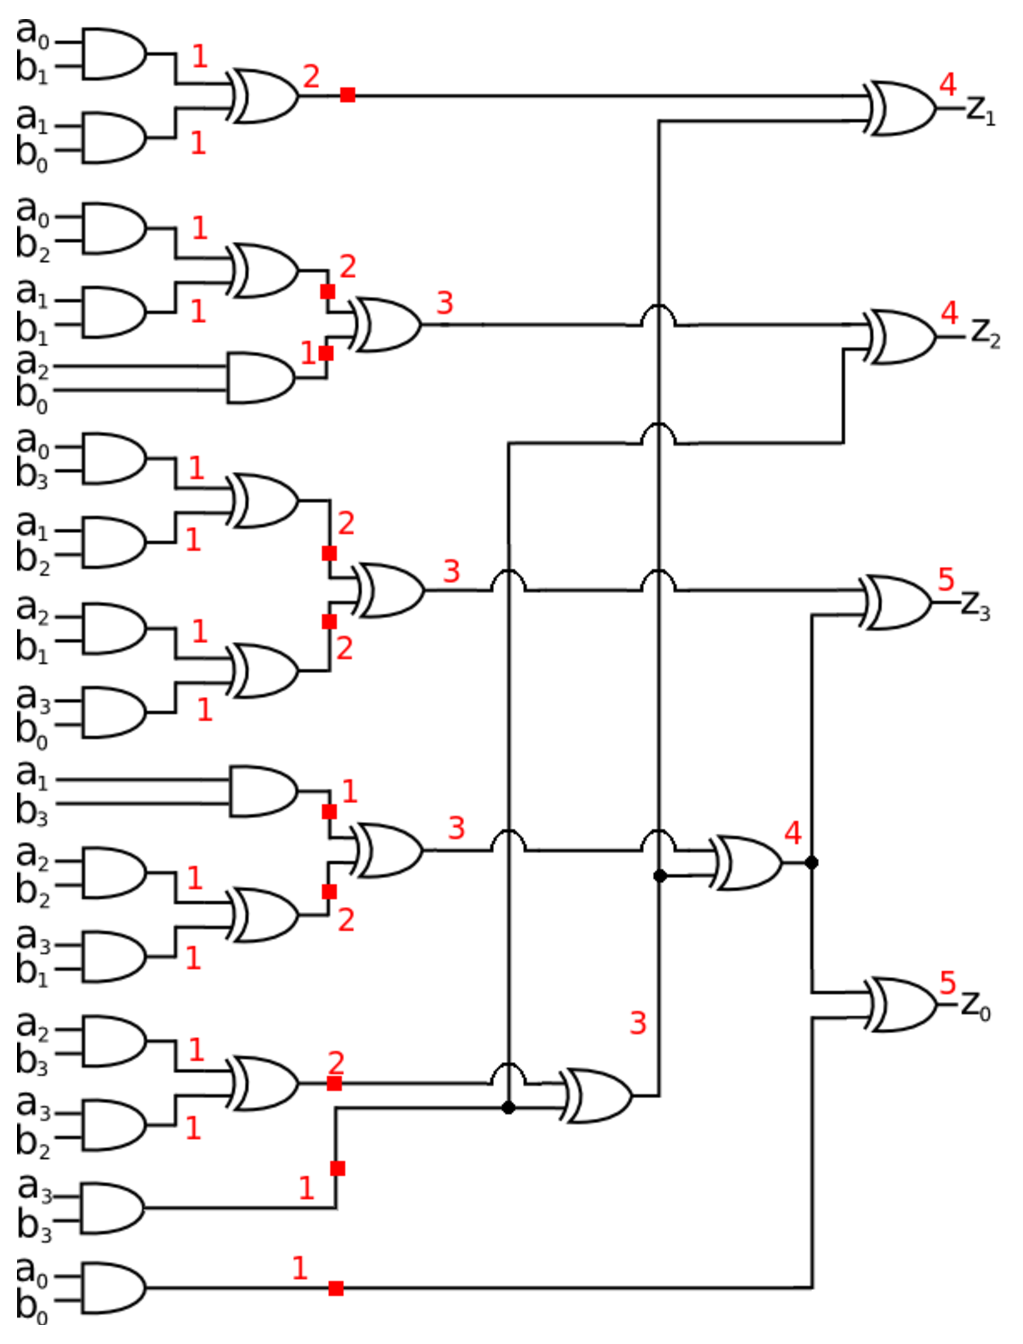
\includegraphics[scale=0.7]{figures/mul4bitTopo2.eps}
	\end{center}
	\caption{Topological Depth and Node Selection}
	\label{fig:nodes}
\end{figure}
\label{exp:mul4topex}
\end{Example}

Now, we the half of the circuit where the nodes $M$ act as the
bit-level outputs.
Select exactly $k$ nodes in $M$, where $k$ is the size of the field $\Fkk$; 
we call these nodes $M_1$. $M_1$ can be considered a $k$-bit word-level 
output. By including every path from $M_1$ to the primary inputs, we 
create a partition $P_1$. Thus, the $k$-bit word-level output of $P_1$ 
are the nodes $M_1$. The $k-bit$ word-level inputs to $P_1$ are the same 
inputs as to the circuit $C$. Thus, $P_1$ is a partition which can be 
analyzed over $\Fkk$.

With $P_1$ designated, select the next $k$ nodes $M_2\subset M$, where $M_2$
contains none of the same nodes as $M_1$. 
Create another partition, $P_2$, where $M_2$ is the $k-bit$ output of $P_2$.
Continue to do this 
until all nodes $M$ have been used in at least one partition.
For the last partition, it is likely that there will be fewer
than $k$ of nodes remaining in $M$ which have not yet been used as the 
output of some partition. 
At this point, select all of the remaining nodes in $M$ which have not been
used
and add in extra nodes in $M$ that have been previously used in a 
partition in order to bring the total to number $k$. Use this collection
of nodes to create the last partition.
Thus, we allow some nodes in $M$ may be outputs of more than one partition, 
although we try to minimize this.
We now have designated $i$ partitions, $P_1 \cdots P_i$, each with a $k$ 
bit output.

\begin{Example}
Refer to the same 4-bit Mastrovito multiplier circuit from Example 
\ref{exp:mul4topex}. We have already found every node $M$. Since $k=4$,
we need to seperate these nodes into groups of $4$ and create partitions
that span from the nodes $M$ to the bit-level inputs 
$\{a_0,\dots,a_3,b_0,\dots,b_3\}$. As there are $10$ nodes in $M$, this will
create $3$ partitions with some nodes in $M$ being
used as the output of more than one partition.

By incrementally selecting $4$ nodes at a time starting at the top, and
labelling the $4$-bit word-level outputs as $H,G,F$, we create partitions
as shown in Figures \ref{fig:part1}, \ref{fig:part2}, and \ref{fig:part3}.

\begin{figure}[H]
	\begin{center}
	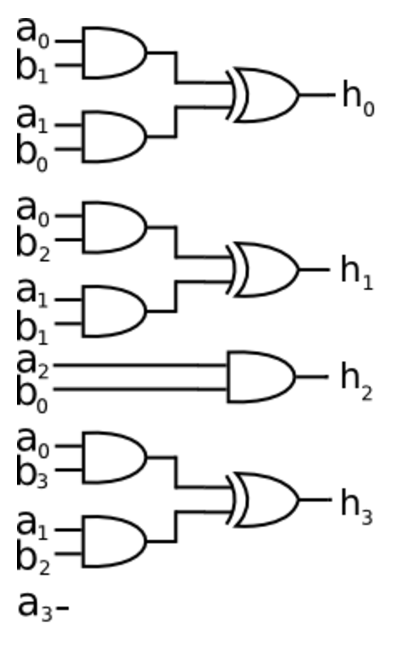
\includegraphics[scale=0.8]{figures/part1.eps}
	\end{center}
	\caption{First Partition, output $H$}
	\label{fig:part1}
\end{figure}

\begin{figure}[H]
	\begin{center}
	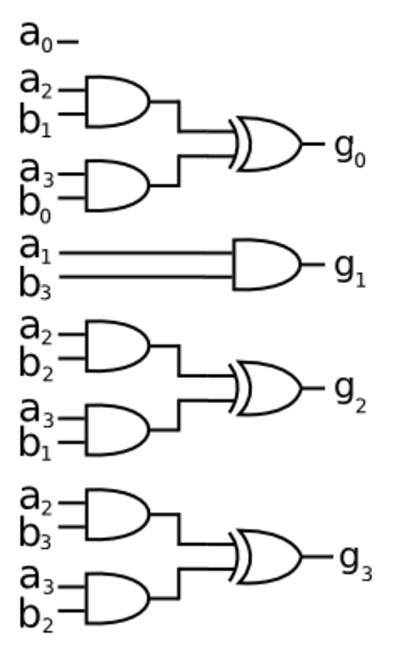
\includegraphics[scale=0.8]{figures/part2.eps}
	\end{center}
	\caption{Second Partition, output $G$}
	\label{fig:part2}
\end{figure}

\begin{figure}[H]
	\begin{center}
	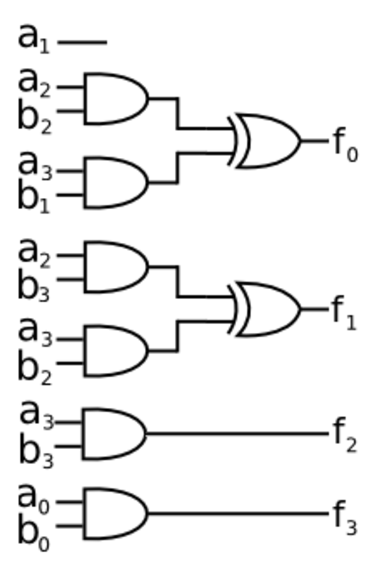
\includegraphics[scale=0.8]{figures/part3.eps}
	\end{center}
	\caption{Third Partition, output $F$}
	\label{fig:part3}
\end{figure}

Note that $f_0=g_2$ and $f_1=g_3$.
\label{exp:mul4inputparts}
\end{Example}

With one half of the circuit partitioned, we look at the other half 
where the nodes in $M$ act as the bit-level inputs. 
The partitions $P_1, \cdots, P_i$ now act as $k$ bit inputs into the second 
half of the circuit. Since there is only one $k$ bit output in the circuit, 
$Z$, we can take the whole second half of the circuit and create one 
partition with $i$ $k$-bit inputs from the outputs of $P_1...P_i$, and one 
$k$ bit output, $Z$. Thus we have partitioned the entire circuit. Since each
partition contains one $k$-bit word-level output and only $k$-bit word-level
inputs, each partition can be analyzed over the same Galois field $\Fkk$ as
the original circuit.

\begin{Example}
Continue the partitioning approach to the 4-bit multiplier
in Example \ref{exp:mul4inputparts}. By using the outputs of the $3$ 
partitions we already have, $\{h_0,\dots,h_1,g_0,\dots,g_3,f_0,\dots,f_3\}$, 
as inputs, we can create the last partition as shown in 
Figure \ref{fig:part4}.

\begin{figure}[H]
	\begin{center}
	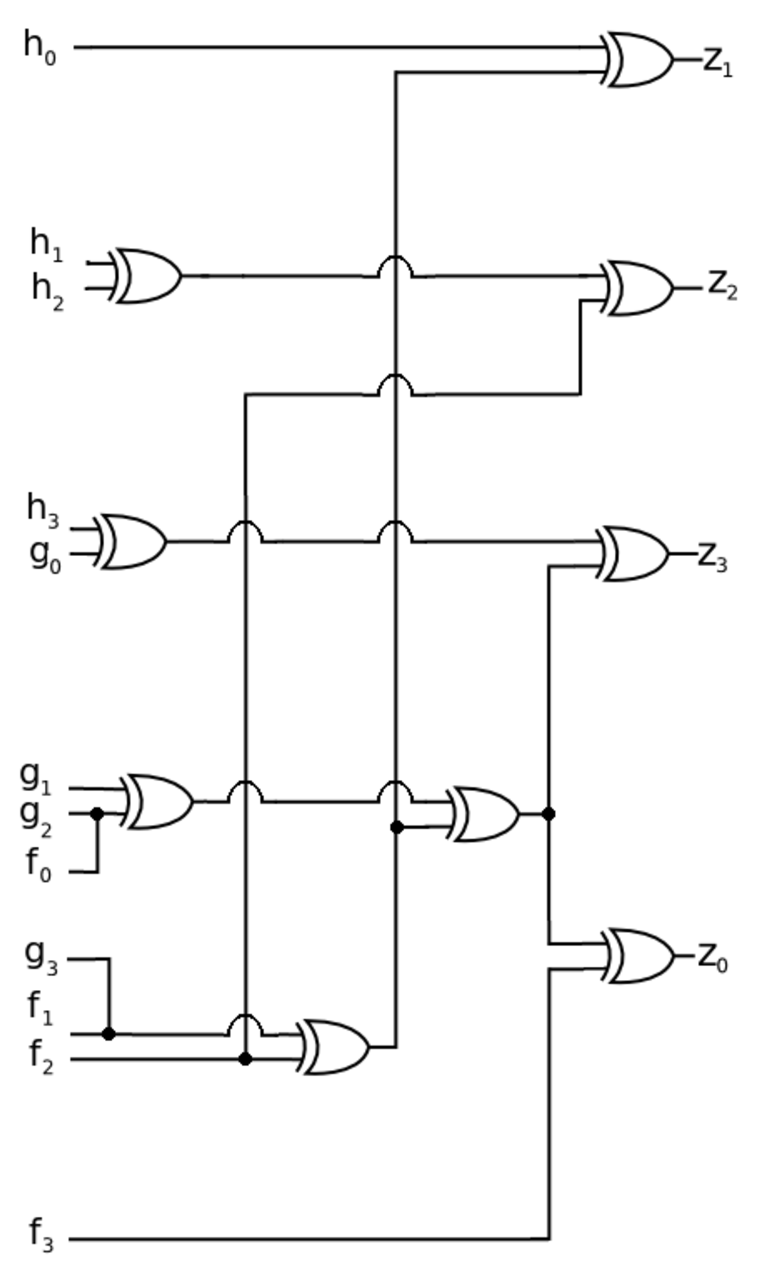
\includegraphics[scale=0.7]{figures/part4.eps}
	\end{center}
	\caption{Fourth Partition}
	\label{fig:part4}
\end{figure}

Thus, the $4$-bit Mastrovito multiplier is fully represented by the four
partitions, as shown in Figure \ref{fig:partitions}.

\begin{figure}[H]
	\begin{center}
	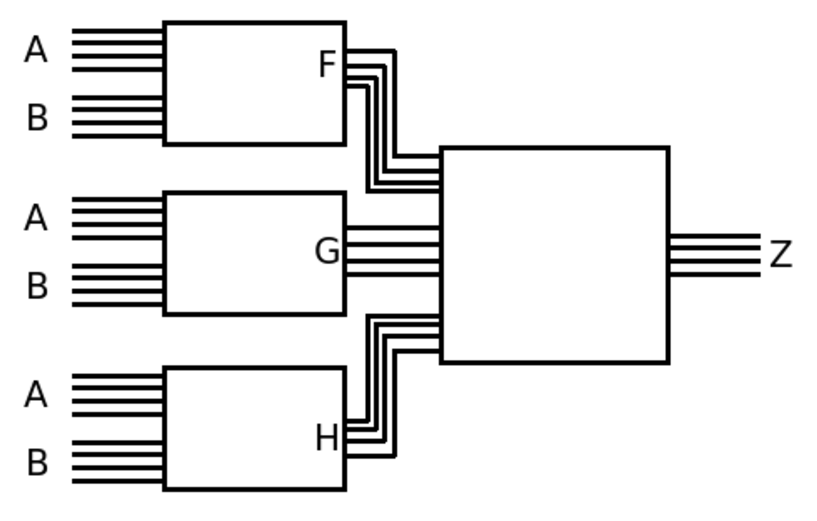
\includegraphics[scale=0.7]{figures/partitions.eps}
	\end{center}
	\caption{Partitioned Circuit Structure}
	\label{fig:partitions}
\end{figure}
\label{exp:mul4partlast}
\end{Example}

\subsection{Overall Approach}
Algorithm \ref{alg:part} is our overall algorithm for creating partitions of 
Galois field arithmetic circuit over $\Fkk$. 

\begin{algorithm}[H]
\SetAlgoNoLine
 \KwIn{$C = $ circuit over $\Fkk$ with $k$ bit input $A$ and $k$ bit output $Z$}
 \KwOut{$P =$ list of circuit partitions}
  $M = $\xspace\{\}\;
  $P = $\xspace\{\}\;
  $D = $ max topological depth of $C$\;
  \For{ every path $T$ in $C$ }
  {
    \For{ every node $N$ in $T$ in reverse topological order }
    {
      \If{ $N \in M$ }
      {
        break\;
      }
      \If{ $N$.depth $<= \frac{D}{2}$ }
      {
        $M = M \cup N$\;
        break\;
      }
    }
  }
  \For{ every $k$ nodes in $M$ as $m_i$ }
  {
  	$P = P$ \xspace$\cup$ partition from $A$ to $m_i$
  }
  $P = P$ \xspace$\cup$ partition from $M$ to $Z$
\caption {General Partitioning Algorithm}\label{alg:part}
\end{algorithm}

Note that while our algorithm proposes to cut the circuit approximately in 
half by finding all nodes of depth $\frac{D}{2}$, this is merely for 
simplicity's sake. This cut can be shifted by changing the depth at which
to search for these nodes. By changing this depth we change the 
relative sizes of the input and output partitions.

\subsection{Applying Abstraction to Circuit Partitions}

Applying abstraction to partitions is similar to applying abstraction to
Montgomery multiplier blocks. We abstract a word-level polynomial 
representation of each partition in parallel. The polynomial abstraction
of the output partition is
\begin{equation}
f_Z: Z + \Func(G_1,\dots,G_i) \nonumber
\end{equation}
where $Z$ is the word-level output of the entire circuit and 
$\{G_1,\dots,G_i\}$ are the word-level outputs of the input partitions
$\{P_1,\dots,P_i\}$. The word-level abstractions of the input partitions are
\begin{eqnarray}
f_1: G_1 + \Func(A_1,\dots,A_n) \nonumber \\
\vdots \\
f_i: G_i + \Func(A_1,\dots,A_n) \nonumber
\end{eqnarray}
where $\{A_1,\dots,A_n\}$.
We are looking for a polynomial in the form of $Z+\Func(A_1,\dots,A_n)$.
Thus, using lex abstraction order $G_1>\dots>G_i>Z>A_1>\dots>A_n$, if we 
perform the reduction $f_Z\stackrel{f_1,\dots,f_i}{\longrightarrow}_+ r$,
$r$ will contain the word-level polynomial $Z+\Func(A_1,\dots,A_n)$.

There are a few issues, however. Every function over $\Fkk$ is a polynomial
function, but for arbitrary logic these polynomial functions can be quite
large. For instance, in $4$-bit multiplier in Example \ref{exp:mul4partlast},
the polynomial word-level abstraction of the partition with output $F$, 
in the form of $F+\Func(A,B)$, is

\begin{eqnarray}
F+(\alpha^3+1)A^8 B^8+(\alpha^2+\alpha)A^8 B^4+A^8 B^2+(\alpha^3+\alpha+1) A^8 B+(\alpha^3+\alpha+1) A^4 B^8 \nonumber \\
+(\alpha+1) A^4 B^4+(\alpha^2+\alpha) A^4 B^2+A^4 B+(\alpha^3+\alpha+1) A^2 B^8+(\alpha^3) A^2 B^2+(\alpha^3+\alpha^2) A B^8 \nonumber \\
+(\alpha^3+\alpha) A B^4+(\alpha^3+\alpha^2) A B^2+(\alpha^3+\alpha+1) A B \nonumber 
\end{eqnarray}

Thus, as the circuit grows in the size, the polynomial abstraction of each
partition will become quite large. This could make reduction time-consuming.
Also, since every partition is random logic over $\Fkk$, our 
abstraction approach that obviates the complexity of \Grobner basis 
computation will always produce a representation that includes bit-
level input variables. Thus, the simple reduction approach shown above will
not work. Thus, in order to seriously consider abstraction with 
partitioning for circuits of applicable sizes, we need to an abstraction 
solution that obviates \Grobner basis complexity and always computes a word-
level representation only.

\section{Analyzing Circuits Over Two Different Galois Fields}

Thus far, our abstraction technique only worked for circuits that perform
a function $\Func$ over $\Fkk$. That is, a circuit which mapped inputs
over $\Fkk$ to outputs over $\Fkk$, $\Func:\Fkk\rightarrow \Fkk$. This
limits the approach only to circuits with inputs and outputs of equal size 
$k$.

In this section, we present a method for abstracting a representation of a
circuit which maps inputs over a field $\F_{2^k}$ to outputs over another
field $F_{2^j}$, where $k \neq j$. 

\subsection{Problem Statement}
A circuit which performs a functional mapping from $\F_{2^k}$ to $\F_{2^n}$
must have $k$-bit word-level inputs and a $j$-bit word-level output. 
Thus, our problem statement is as follows:

\begin{itemize}
\item Given a Galois field $\F_{2^k}$, i.e. given the corresponding
irreducible polynomial $P_k(x)$ in $\F[x]$ of degree $k$,
let $P_k(\beta) = 0$ where $\beta \in \F_{2^k}$ is the root of the 
irreducible polynomial $P_k$.
\item Given another Galois field $\F_{2^j}$, where $j\neq k$, i.e. 
given the corresponding
irreducible polynomial $P_j(x)$ in $\F[x]$ of degree $j$,
let $P_j(\gamma) = 0$ where $\gamma \in \F_{2^j}$ is the root of the 
irreducible polynomial $P_j$.
\item Given another Galois field $\F_{2^h}$, where $h=lcm(j,k)$, i.e. 
given the corresponding
irreducible polynomial $P_h(x)$ in $\F[x]$ of degree $h$,
let $P_h(\alpha) = 0$ where $\alpha \in \F_{2^h}$ is the root of the 
irreducible polynomial $P_h$.
\item Given a gate-level combinational circuit $C$ with
word-level $k$-bit input $A \in \Fkk$, and
and $j$-bit output $Z \in \F_{2^j}$.
\item The bit-level primary input of the circuit is denoted
$\{a_0,\dots,a_{k-1}\} \in \F_2$,
the primary bit-level outputs are $\{z_0, \dots, z_{j-1}\} \in \F_2$.
\item The word-level primary input is denoted 
$A = a_0 + a_1\beta + \dots + a_{k-1}\beta^{k-1}$ and the word-level 
primary output is denoted $Z = z_0 + z_1\gamma + \dots + z_{j-1}\gamma^{j-1}$
\item Find the word-level polynomial function $\Func$ over $\F_{2^h}$
performed by $C$ in the form of $Z=\Func(A_1, \dots, A_n)$.
\end{itemize}

Since the word-level inputs $\{A_1, \dots, A_n\} \in \Fkk$ and the
word-level output $Z \in \F_{2^j}$, the abstraction polynomial 
$Z+\Func(A_1, \dots, A_n)$ must be in $\F_{2^h}$ where 
$\Fkk \subset \F_{2^h}$ and $\F_{2^j} \subset \F_{2^h}$. In other words,
the word-level polynomial is contained in the smallest field that contains 
both the input field $\Fkk$ and output field $\F_{2^j}$. Thus, $h=lcm(k,j)$.

\subsection{Problem Formulation}

Since the abstraction polynomial representation is over the field 
$\F_{2^h}$, we need to model the entire circuit as a system of polynomials 
over this field (as shown in our abstraction chapter).
The only polynomials that cannot be 
immediately modelled over this field are the word-level designation 
polynomials, $f_A$ and $f_Z$.
\begin{eqnarray}
f_A&:&a_0 + a_1\beta + \dots + a_{k-1}\beta^{k-1} \nonumber \\
f_Z&:&z_0 + z_1\gamma + \dots + z_{j-1}\gamma^{j-1} \nonumber
\end{eqnarray}
$f_A$ and $f_Z$ have coefficients $\beta$ and $\gamma$
which are over $\Fkk$ and $\F_{2^j}$ respectively.
Thus, we need to represent $\beta$ and $\gamma$ in terms of 
$\alpha \in \F_{2^h}$.
For this, we
use the following result from \cite{cf:2003} related to 
{\bf composite fields}, which states the following:

\begin{Theorem}
Let $k = m\cdot n$, such that $\Fkk = \F_{(2^m)^n}$. Let $\alpha$ be
the primitive root of $\F_{(2^m)^n}$, and let $\beta$ be the
primitive root of the ground field $\F_{2^m}$. Then,
$\beta=\alpha^{\omega}$, where $\omega=(2 ^{m \cdot n}-1)/(2^m-1)$. 
In other words: 
\begin{equation}
\beta=\alpha^{(2^{m \cdot n}-1)/(2^m-1)} \nonumber
\label{eqn:relation}
\end{equation}
\label{thm:2to3thm}
\end{Theorem}
Since $h=lcm(k,j)$, there exists a $m$ such that $h = k\cdot m$.
Likewise, there exists a $n$ such that $h = j\cdot n$.
Thus, using the above theorem, we can find $\beta = \alpha^\omega$ and 
$\gamma = \alpha^\psi$, where
\begin{eqnarray}
\omega = (2^{k \cdot m}-1)/(2^k-1) \nonumber \\
\psi = (2^{j \cdot n}-1)/(2^j-1) \nonumber 
\end{eqnarray}
Thus, we can write $A$ and $Z$ in terms of $\alpha$ as follows:
\begin{eqnarray}
A = a_0+a_1\cdot\alpha^\omega+\dots+a_{k-1}\cdot\alpha^{(k-1)\omega} \nonumber \\
Z = z_0+z_1\cdot\alpha^\psi+\dots+z_{j-1}\cdot\alpha^{(j-1)\psi} \nonumber
\end{eqnarray}

\begin{Example}
Consider the following circuit shown in Figure \ref{fig:2to3fig}.
\begin{figure}[H]
	\begin{center}
	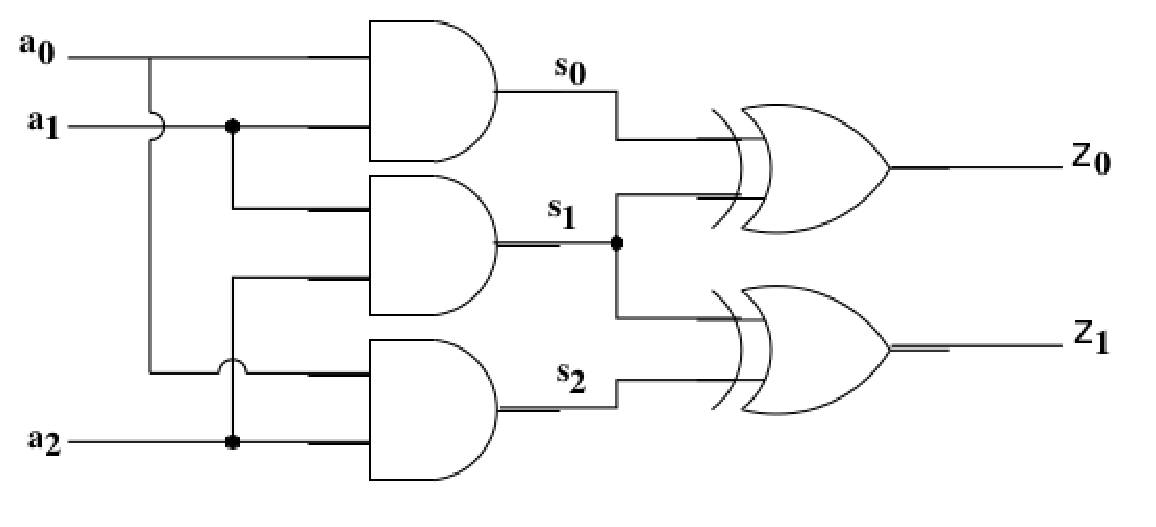
\includegraphics[scale=0.80]{figures/2to3.eps}
	\end{center}
	\caption{Circuit with function $\F_{2^3} \rightarrow \F_{2^2}$}
	\label{fig:2to3fig}
\end{figure}

This circuit has a $3$-bit input $A$ and a $2$-bit output $Z$. Thus, it can
be considered to be a functional mapping over two fields 
$\F_{2^3} \rightarrow \F_{2^2}$. Let $\beta$ be the root of the irreducible 
polynomial $P_k$ of degree $3$ which is generates $\F_{2^3}$. 
Let $\gamma$ be the root of
the irreducible polynomial $P_j$ of degree $2$
which generates $\F_{2^2}$. Then the 
word-level designation polynomials of the input and output, $f_A$ and $f_Z$, 
are:
\begin{eqnarray}
f_A&:&A+a_0+a_1\cdot\beta+a_2\cdot\beta^2 \nonumber \\
f_Z&:&Z+z_0+z_1\cdot\gamma \nonumber
\end{eqnarray}

As $lcm(2,3)=6$, the smallest field that contains both 
$\F_{2^3}$ and $\F_{2^2}$ is $\F_{2^6}$. Thus,
the word-level polynomial $Z+\Func(A)$ is a polynomial over $\F_{2^6}$.
Let $\alpha$ be the root of the 
irreducible polynomial $P_h$ of degree $6$ which generates $\F_{2^6}$. 
Using Theorem \ref{thm:2to3thm}, we find $\beta$ and $\gamma$ in terms of 
$\alpha$, as follows: 
\begin{eqnarray}
\beta=\alpha^\omega, \omega={2^{2\cdot3}-1 \over 2^3-1}=9 \nonumber \\
\gamma=\alpha^\psi, \psi={2^{3\cdot2}-1 \over 2^2-1}=21 \nonumber
\end{eqnarray}
thus, $\beta=\alpha^9$ and $\gamma=\alpha^{21}$. 
The polynomials $f_A$ and $f_Z$ are now be represented as:
\begin{eqnarray}
f_A&:&A+a_0+a_1\cdot\alpha^9+a_2\cdot\alpha^{18} \nonumber \\
f_Z&:&Z+z_0+z_1\cdot\alpha^{21} \nonumber
\end{eqnarray}
We can now analyze the entire circuit over $\F_{2^6}$.
\label{exp:2to3ex1}
\end{Example}

\subsection{Abstraction of Circuits over Different Galois Fields}

With all polynomials modelled over $\F_{2^h}$, we can apply our abstraction
approach using abstraction ordering to find the word-level polynomial
function $Z+\F(A)$ over $\F_{2^h}$, as shown in a previous chapter. Note that
vanishing polynomials for the word-level variables, $A$ and $Z$ are formed 
from their corresponding fields, i.e. $A^{2^k}-A$ and $Z^{2^j}-Z$.

\begin{Example}
Consider the same circuit from Example \ref{exp:2to3ex1}, which performs a
function $\F_{2^3} \rightarrow \F_{2^2}$.
Let $\alpha$ be the root of the irreducible polynomial $P_h=X^6+X+1$, which
is used to construct $\F_{2^6}$.
We model the entire circuit as a system of polynomials $J$ over $\F_{2^6}$.
We find the relevant vanishing polynomials $J_0$. Abstraction ordering of 
this circuit is
\begin{equation}
z_0>z_1>s_0>s_1>s_2>a_0>a_1>a_2>Z>A \nonumber
\end{equation}
The system of polynomials $J+J_0$ is

\begin{eqnarray}\label{eqn:miterbit}
 \left .  \begin{aligned}
f_1&:&s_0+a_0\cdot a_1\nonumber\\
f_2&:&s_1+a_1\cdot a_2\nonumber\\
f_3&:&s_2+a_0\cdot a_2\nonumber\\
f_4&:&z_0+s_0+s_1\nonumber\\
f_5&:&z_1+s_1+s_2\nonumber\\
\end{aligned}
\ \right\}
&\qquad&  \text{\it Bit-level implementation} (J) \nonumber \\
 \left .  \begin{aligned}
f_A&:&a_0+a_1\cdot\alpha^9+a_2\cdot\alpha^{18}+A\nonumber\\
f_Z&:&z_0+z_1\cdot\alpha^{21}+Z\nonumber\\ 
\end{aligned}
\ \right\}
 &\qquad&  \text{\it Word-level designation} (J) \nonumber \\
\left . \begin{aligned}
a_0^2-a_0\nonumber\\
a_1^2-a_1\nonumber\\
a_2^2-a_2\nonumber\\
z_0^2-z_0\nonumber\\
z_1^2-z_1\nonumber\\
s_0^2-s_0\nonumber\\
s_1^2-s_1\nonumber\\
s_2^2-s_2\nonumber\\
A^8-A\nonumber\\
Z^4-Z\nonumber
\end{aligned}
\ \right\}
&\qquad&  \text{\it Vanishing Polynomials} (J_0) \nonumber 
\end{eqnarray}

By computing a reduced \Grobner basis, the word-level abstraction polynomial
in the form of $Z+\Func(A)$ is found in the basis:
\begin{equation}
Z+(\alpha^2+\alpha)A^6+(\alpha^4+\alpha^3+\alpha)A^5+(\alpha^2+\alpha)A^4+(\alpha^4+\alpha^3+\alpha^2)A^3+(\alpha^4+\alpha^3+\alpha^2)A^2+(\alpha^4+\alpha^3+\alpha)A \nonumber
\end{equation}
\end{Example}


This method allows us to abstract a word-level polynomial representation
of circuits which have inputs and outputs of different datapath sizes, where
previously abstraction was only possible if the datapath of the inputs and
outputs was the same.
However, if this circuit with function $\Fkk \rightarrow \F_{2^j}$ does not 
perform a
simple function over the give $\F_{2^h}$, like in the example above, then 
the word-level polynomial representation over $Z+\Func(A)$ over $\F_{2^h}$ 
could be quite large. In this case, our approach to obviate the complexity
of the \Grobner basis computation will derive a representation with bit-level
input variables.
Also, depending on the size of the inputs, $k$, and the 
size of the outputs, $j$, the field $\F_{2^h}$ could be very large if $j$ and
$k$ are relatively prime to each other, i.e. $lcm(j,k)=j*k$.

\section{Conclusions}

In this chapter we proposed two more applications of word-level abstraction 
over Galois Fields: a partitioning algorithm over $\Fkk$ and an approach to
analyze circuits over $\Fkk \rightarrow \F_{2^j}$.
Notably, these proposals are applicable not just to 
abstraction, but to all computer-algebra based formal verification of Galois 
field circuits. Currently, there are a few limitations of these proposals 
when applied to our abstraction approach. When applied to partitions, our 
abstraction approach with obviation of \Grobner basis computation produces a 
result with bit-level input variables. Thus, we cannot apply substitution to
abstract the full representation of the partitioned circuit. However, 
we could potentially apply these mixed-level abstractions to Lv's
equivalence approach, as described in the previous chapter.

There are a number of unexplored applications of the proposals put forth in 
this chapter. If our abstraction approach could guarantee a word-level 
abstraction of any circuit logic, then the partitioning approach could 
very-well allows us to abstract even larger Galois field circuits. Our 
proposal of abstracting representations of circuits over 
$\Fkk \rightarrow \F_{2^j}$ could also then be applied to allow for 
partitions of varying inputs and outputs. These applications seem 
promising, and thus motivate further research.
